\documentclass[10pt,twocolumn]{article}
\usepackage[margin=0.8in,columnsep=0.25in]{geometry}
\usepackage[T1]{fontenc}
\usepackage{lmodern}
\usepackage{microtype}
\usepackage{amsmath}
\usepackage{booktabs}
\usepackage{graphicx}
\usepackage{xcolor}
\usepackage{tikz}
\usetikzlibrary{positioning,arrows.meta,fit}
\usepackage[font=small,labelfont=bf]{caption}
\usepackage{enumitem}
\setlist{nosep,leftmargin=*}
\usepackage[hidelinks]{hyperref}
\usepackage{url}

\newcommand{\idleMedian}{15.9}
\newcommand{\nTrials}{38}


\title{Fair Queueing Is Not Enough at Flow Start:\\
\large Game-Grade Latency on a Marginal VDSL2 Line with a One-Armed CAKE Router}
\author{Emmet\\\small\url{https://github.com/Emmet-v15/one-armed-cake}}
\date{September 2026}

\begin{document}
\maketitle

\begin{abstract}
We report a measurement study of latency under load on a residential VDSL2
line with roughly 5.9\,Mbit/s down and 2\,Mbit/s up, where the ISP router cannot
be modified. A Raspberry Pi~4B attached to one LAN port acts as a
\emph{one-armed} router and shapes both directions with CAKE. We make four
observations. (i)~Shaping both directions on \emph{egress}, after NAT, is what
makes per-host fairness possible on such a box, and CAKE's \texttt{nat} option
is required on the upload side. (ii)~Fair queueing does not protect a sparse,
game-like flow while many bulk flows are \emph{starting}: with 16 simultaneous
uploads, a 50\,Hz UDP probe saw worst-case round trips of 97--132\,ms and lost
13\% of its packets in the first 1.5\,s, even though CAKE was the only queue
involved. Classifying small UDP packets into CAKE's Voice tin removed the effect
entirely (22--40\,ms, no loss). (iii)~Capping download at 4.5\,Mbit/s keeps
steady-state latency at a median of 18\,ms and a p99 of 26\,ms, compared with 165\,ms and 229\,ms unshaped,
but it cannot stop a ${\sim}$120\,ms p99 transient when a download starts. This is a basic
limit of shaping at the receiving end. (iv)~Several common measurement methods were misleading on this
line: ICMP is policed upstream, TCP-handshake probes turn a single loss into a
1\,s sample, and one load generator was throttled on the client host.
All code, configuration, and raw data are released.
\end{abstract}

\section{Introduction}
Bufferbloat, excessive queueing delay in oversized network buffers, remains the
dominant cause of latency spikes on residential links~\cite{gettys2011}. Modern
active queue management (AQM) such as CoDel~\cite{codel,rfc8289},
FQ-CoDel~\cite{rfc8290}, and CAKE~\cite{cake} solves it when it runs at the
bottleneck. The ISP-supplied router usually sits at the bottleneck, and it
usually cannot run custom AQM.

This paper documents what it takes to get \emph{game-grade} latency (a steady
round trip well under 50\,ms while other devices saturate the line) on such a line,
using a single-board computer that sits beside the ISP router rather than in
front of it. The line is marginal: VDSL2 at ${\sim}$88\,dB downstream
attenuation, SNR margins of 6.6/5.4\,dB, and a delivered capacity that drifted
between 2.3 and 5.9\,Mbit/s over the study.

\paragraph{Contributions.}
\begin{itemize}
\item A \textbf{one-armed shaper design} that shapes both directions on egress,
  after NAT, so that CAKE's per-host isolation works in both directions. We
  show why the ingress hook cannot do this and why CAKE's \texttt{nat} keyword
  is required on the upload side (\S\ref{sec:design}).
\item A \textbf{measurement method} for such a box: a game-style UDP probe to a
  reflector we control, plus packet-level localization using the fact that each
  packet crosses the router's single interface four times (\S\ref{sec:method}).
\item \textbf{Flow-startup vulnerability of fair queueing}: we quantify it and
  show that a simple size-based classifier eliminates it (\S\ref{sec:upload}).
\item A \textbf{download cap sweep} that separates steady-state control, which
  works, from the flow-start transient, which receiver-side shaping cannot
  remove (\S\ref{sec:download}).
\item \textbf{Negative results and pitfalls}: priority by demotion, ICMP-driven
  autorate, and probe and load-generator artifacts (\S\ref{sec:pilot},
  \S\ref{sec:pitfalls}).
\end{itemize}

\section{Background}
CoDel~\cite{codel,rfc8289} drops or marks packets when their queueing delay
(\emph{sojourn time}) has exceeded a \emph{target} for at least an
\emph{interval}. FQ-CoDel~\cite{rfc8290} hashes packets into per-flow queues
with a CoDel instance each, and serves flows by deficit round robin. Flows that
have just become active are kept on a separate ``new flows'' list, which is
served first. This \emph{sparse-flow optimization} is what normally gives
low-rate interactive traffic its low latency.

CAKE~\cite{cake} builds on this with a deficit-mode shaper, per-host fairness
(\texttt{dual-srchost}/\texttt{dual-dsthost}), DiffServ \emph{tins} (in
\texttt{diffserv4}: Bulk, Best Effort, Video, Voice; Voice is prioritized up to
a 25\% bandwidth threshold), an \texttt{ingress} mode for shaping at the
receiving side, an ACK filter, and link-layer overhead compensation.

Shaping download on the \emph{receiving} side is inherently indirect: the real
bottleneck buffer is upstream, at the DSLAM. The shaper can only keep that buffer
empty by delivering slightly less than line rate and dropping packets, which
signals senders one round trip later. cake-autorate~\cite{autorate} adjusts
the shaper rate continuously from ICMP round-trip measurements.

\section{System Design}\label{sec:design}
\begin{figure}[t]
\centering
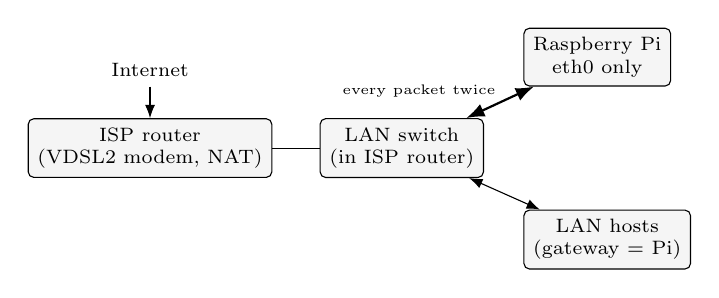
\begin{tikzpicture}[node distance=6mm and 6mm, every node/.style={font=\scriptsize},
  box/.style={draw,rounded corners=2pt,minimum height=6mm,align=center,fill=gray!8}]
\node[box] (isp) {ISP router\\(VDSL2 modem, NAT)};
\node[box,right=of isp] (sw) {LAN switch\\(in ISP router)};
\node[box,above right=4mm and 5mm of sw] (pi) {Raspberry Pi\\eth0 only};
\node[box,below right=4mm and 5mm of sw] (pc) {LAN hosts\\(gateway = Pi)};
\node[above=4mm of isp] (inet) {Internet};
\draw[-{Latex}] (inet) -- (isp);
\draw (isp) -- (sw);
\draw[{Latex}-{Latex},thick] (sw) -- node[above left=-1mm,font=\tiny]{every packet twice} (pi);
\draw[{Latex}-{Latex}] (sw) -- (pc);
\end{tikzpicture}

\vspace{3mm}
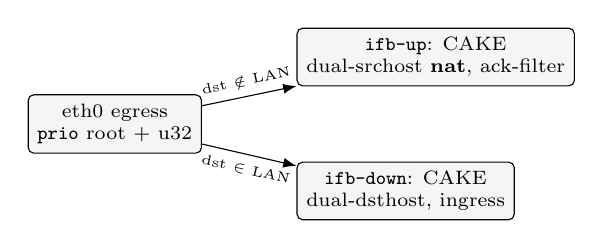
\begin{tikzpicture}[node distance=3mm and 4mm, every node/.style={font=\scriptsize},
  box/.style={draw,rounded corners=2pt,minimum height=5mm,align=center,fill=gray!8}]
\node[box] (e) {eth0 egress\\\texttt{prio} root + u32};
\node[box,above right=1mm and 12mm of e] (up) {\texttt{ifb-up}: CAKE\\dual-srchost \textbf{nat}, ack-filter};
\node[box,below right=1mm and 12mm of e] (dn) {\texttt{ifb-down}: CAKE\\dual-dsthost, ingress};
\draw[-{Latex}] (e) -- node[above,font=\tiny,sloped]{dst $\notin$ LAN} (up);
\draw[-{Latex}] (e) -- node[below,font=\tiny,sloped]{dst $\in$ LAN} (dn);
\end{tikzpicture}
\caption{Top: one-armed topology. The Pi serves DHCP and names itself as the
gateway, so all traffic hairpins through its single port. Bottom: both
directions are classified on eth0 egress and redirected to per-direction CAKE
instances. LAN-to-LAN traffic bypasses shaping.}
\label{fig:topo}
\end{figure}

\paragraph{Topology.} The Pi (static 192.168.1.2) runs dnsmasq and hands out
itself as the default gateway; the ISP router's own DHCP server is disabled
(Fig.~\ref{fig:topo}). The Pi masquerades to the ISP router, which NATs again
to the Internet. Every forwarded byte crosses the Pi's 1\,GbE link twice, which
is negligible at these rates.

\paragraph{Why egress, both directions.} A tc ingress hook sees inbound packets
before conntrack reverses NAT, so every download packet is still addressed to
the router itself. Per-host fairness is impossible there. On egress towards the
LAN, the destination is the real host. On egress towards the ISP router, however, the
source has \emph{already} been masqueraded: counting in a postrouting chain at
priority~200 showed 7{,}600 packets from the router's address and none from the
real host. CAKE's \texttt{nat} option, which recovers the pre-NAT address from
conntrack, is therefore load-bearing on the upload side: without it,
\texttt{dual-srchost} sees one host and isolates nothing. Download needs no
\texttt{nat}. A \texttt{prio} root with three u32 filters sends LAN$\to$LAN traffic
unshaped, traffic to a LAN destination to \texttt{ifb-down}, and everything else to
\texttt{ifb-up}.

\paragraph{Profiles.} \emph{Gaming} caps download at 4.5\,Mbit/s with CAKE
\texttt{rtt 30ms}. \emph{Max} leaves download \texttt{unlimited}; CAKE still
provides flow isolation and statistics. Upload is capped at 1.8\,Mbit/s in both
(sync 2.0\,Mbit/s), with PTM overhead compensation (\texttt{overhead 34 mpu 68
ptm}) and the ACK filter. Profiles switch at run time with
\texttt{tc qdisc change}, which keeps queued packets and counters.

\paragraph{Game-packet classifier.} An nftables rule in the \texttt{forward}
hook, where real hosts are visible in both directions, sets DSCP EF on
\begin{itemize}
\item LAN-originated UDP packets of $\le$300\,bytes, and
\item LAN-bound UDP packets of $\le$1000\,bytes not from port 443.
\end{itemize}
EF maps to CAKE's Voice tin. The port-443 exclusion keeps QUIC data out, and
the Voice tin's 25\% threshold bounds any misclassification. Upload uses
\texttt{wash} so the mark is not leaked upstream.

\paragraph{Monitoring.} A Bun dashboard reads per-direction byte counters from
sysfs at 20\,Hz and per-host counters from nftables dynamic sets at 1\,Hz. It
measures latency with the same 10\,Hz game-style UDP echo used in
\S\ref{sec:method}, marked EF.

\section{Methodology}\label{sec:method}
\paragraph{Testbed.} Raspberry Pi~4B, Debian~13, Linux 6.18, \texttt{sch\_cake}.
The client is a Windows~11 PC on wired 1\,GbE. The reflector is a cloud VM with a
median idle round trip of \idleMedian\,ms from the client.

\paragraph{Probe.} Each trial sends a UDP datagram with a 64-byte payload
(92-byte IP packet) every 20\,ms, carrying an 8-digit sequence number. The
reflector echoes datagrams of $\le$128\,bytes. A probe with no echo by the end of
the trial counts as lost. This resembles a game's input stream in size and rate,
unlike ICMP (policed on this path, \S\ref{sec:pitfalls}) or TCP handshakes.

\paragraph{Trials.} Each trial is 2\,s idle, then 8\,s of load, then 2\,s idle.
We report the \emph{start} window (the first 1.5\,s of load) and the
\emph{steady} window (the rest of the load) separately. Upload load is $N$ TCP
streams to a sink on the reflector. Download load is 4~curl processes fetching
a public 100\,MB file. Conditions are interleaved within each repetition
(5~repetitions for upload, 3 for download, \nTrials{} trials in total), so
capacity drift affects all conditions alike. Tables report, per condition, the
median across repetitions with the min--max range in parentheses.

\paragraph{Localization.} On a one-armed router a packet crosses eth0 four
times: from the client (A), towards the ISP router after the upload qdisc (B),
the reply from the ISP router (C), and towards the client after the download
qdisc (D). A single \texttt{tcpdump} on eth0, matching packets by payload
sequence number and direction by MAC address, separates time in the upload qdisc
($B-A$), everything beyond the router ($C-B$), and time in the download qdisc
($D-C$), and pinpoints where each lost packet disappeared.

\section{Results}
\subsection{Upload: fair queueing at flow start}\label{sec:upload}

\begin{table*}[t]
\centering\small
\begin{tabular}{rl rrr rrr}
\toprule
& & \multicolumn{3}{c}{load start (first 1.5\,s)} & \multicolumn{3}{c}{steady load} \\
\cmidrule(lr){3-5}\cmidrule(lr){6-8}
flows & marking & median & max & lost & median & p99 & lost \\
\midrule
4 & none & 19 (18--20) & 32 (24--43) & 0/375 & 19 (18--19) & 23 (22--35) & 0/1625 \\
4 & EF & 19 (18--20) & 25 (23--30) & 0/375 & 19 (19--19) & 23 (23--29) & 0/1625 \\
16 & none & 39 (28--42) & 131 (97--132) & 49/375 & 26 (25--32) & 67 (61--87) & 239/1625 \\
16 & EF & 19 (18--20) & 24 (22--40) & 0/375 & 19 (19--20) & 23 (22--33) & 0/1625 \\
\bottomrule
\end{tabular}
\caption{Game-style probe round trip (ms) while $N$ TCP uploads start
simultaneously; upload capped at 1.8\,Mbit/s. ``EF'' = small-UDP classifier on.
Lost = probes lost / probes sent, summed over 5~repetitions.}
\label{tab:upload}
\end{table*}

\begin{figure}[t]
\centering
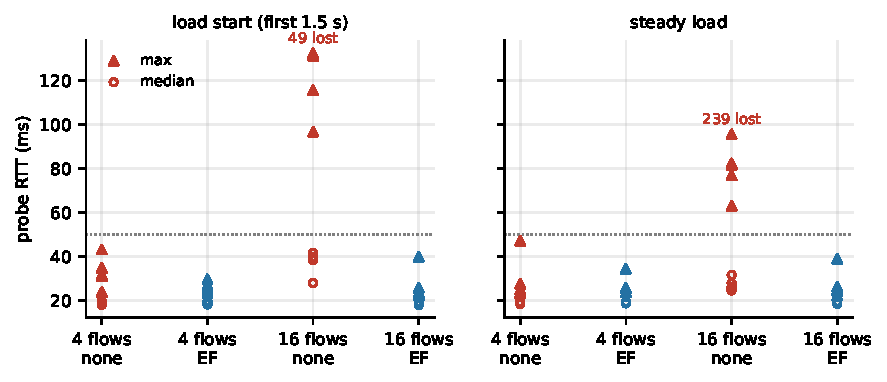
\includegraphics[width=\columnwidth]{figures/upload-start.pdf}
\caption{Per-trial median ($\circ$) and maximum ($\triangle$) probe round trip.
Red: no classifier; blue: small UDP in the Voice tin. Dotted line: 50\,ms.}
\label{fig:upload}
\end{figure}

With 4 uploads, fair queueing alone works: the start-window maximum is
24--43\,ms and there is no loss (Table~\ref{tab:upload}). With 16 uploads it
does not: the median probe round trip doubles to 39\,ms, the worst case reaches
97--132\,ms, and 49 of 375 probes (13\%) are lost in the first 1.5\,s. The
effect persists into steady state (p99 61--87\,ms, 239/1625 lost). With the
classifier on, the 16-flow case is indistinguishable from the 4-flow case:
maximum 22--40\,ms and no loss in any trial (Fig.~\ref{fig:upload}).

\begin{table}[t]
\centering\small
\begin{tabular}{l rr rr}
\toprule
& \multicolumn{2}{c}{upload qdisc} & \multicolumn{2}{c}{beyond router}\\
\cmidrule(lr){2-3}\cmidrule(lr){4-5}
16 uploads & max & lost & median & max\\
\midrule
unmarked, start  & 75.4 & 8  & 15.7 & 17.0\\
unmarked, steady & 51.8 & 11 & 15.6 & 23.2\\
EF, start        & 6.6  & 0  & 15.7 & 17.3\\
EF, steady       & 7.4  & 0  & 15.6 & 24.4\\
\bottomrule
\end{tabular}
\caption{Packet-level localization (ms; one trial per condition). No probe was
lost beyond the router or in the download qdisc.}
\label{tab:local}
\end{table}

\paragraph{Where the delay and loss occur.} Packet capture
(Table~\ref{tab:local}) places all of it inside CAKE's upload qdisc on the Pi.
The ISP router, line, and Internet path stayed flat at 15.6\,ms, and every lost
probe disappeared between A and B. Lowering the upload cap to 1.6 or
1.4\,Mbit/s did not help, which rules out a hidden queue in the ISP router.

\paragraph{Mechanism.} We did not instrument the scheduler directly, but the
data are consistent with the following explanation. When 16 flows start
together, each one is ``new'' in the DRR sense, so the probe no longer has the
new-flow list to itself and waits its turn behind up to 16 quanta. At
1.8\,Mbit/s one 1514-byte quantum takes 6.7\,ms, which bounds the wait at
$16 \times 6.7 \approx 108$\,ms, above the observed in-qdisc maximum of
75\,ms. Meanwhile CAKE's aggregate backlog peaked at ${\sim}$1.15\,s of data.
Probe packets that wait longer than CoDel's target for longer than an interval
make the probe's own CoDel instance drop them, which would explain losses that
occur only inside the qdisc. EF classification moves the probe into the Voice
tin, which is served before Best Effort, and the effect disappears.

\subsection{Download: steady state versus flow start}\label{sec:download}

\begin{table*}[t]
\centering\small\setlength{\tabcolsep}{4.5pt}
\begin{tabular}{lrl rrr rrr r}
\toprule
& & & \multicolumn{2}{c}{load start} & & \multicolumn{3}{c}{steady load} & \\
\cmidrule(lr){4-5}\cmidrule(lr){7-9}
cap (kbit/s) & rtt & mark & median & p99 & & median & p99 & lost & goodput \\
\midrule
unlimited & 100 & EF & 149 (137--161) & 209 (203--213) & & 165 (161--174) & 229 (228--230) & 70/975 & 4.28 (4.27--4.29) \\
5300 & 30 & EF & 154 (133--155) & 197 (196--204) & & 162 (162--169) & 219 (211--221) & 49/975 & 4.65 (4.63--4.68) \\
5100 & 30 & EF & 129 (127--140) & 187 (171--209) & & 23 (21--61) & 208 (178--231) & 14/975 & 3.28 (3.04--3.47) \\
4800 & 30 & EF & 25 (25--25) & 153 (143--172) & & 21 (20--22) & 70 (46--109) & 0/975 & 2.46 (2.06--3.05) \\
4500 & 30 & EF & 22 (22--23) & 124 (111--132) & & 18 (18--19) & 26 (26--35) & 0/975 & 2.80 (2.78--3.02) \\
4500 & 30 & none & 22 (22--55) & 130 (129--137) & & 20 (20--20) & 50 (49--98) & 0/975 & 2.66 (2.40--2.69) \\
\bottomrule
\end{tabular}
\caption{Probe round trip (ms) under 4-stream download, by download cap (wire
rate) and CAKE \texttt{rtt}. Goodput is averaged over the whole 8\,s load period,
including slow start, so it understates steady-state rate.}
\label{tab:download}
\end{table*}

\begin{figure}[t]
\centering
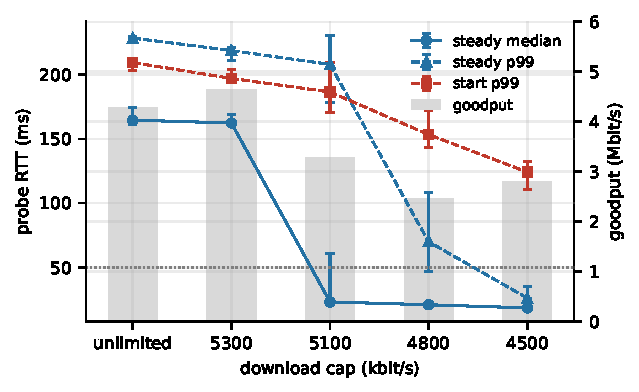
\includegraphics[width=\columnwidth]{figures/download-sweep.pdf}
\caption{Download cap sweep (classifier on). Lines: steady median, steady p99
and start p99 (bars: min--max over repetitions). Grey bars: goodput.}
\label{fig:download}
\end{figure}

Unshaped, the DSLAM buffer fills and the probe sees a median of 165\,ms, a p99 of
229\,ms, and 7\% loss in steady state (Table~\ref{tab:download},
Fig.~\ref{fig:download}). An independent web-based test agreed: +173\,ms under
download, +7\,ms under upload. A 5.3\,Mbit/s cap was above that day's capacity
and behaved like no cap. 5.1\,Mbit/s was at the knee and bimodal. At
4.8\,Mbit/s and below, CAKE owns the queue: at 4.5\,Mbit/s the steady median is
18\,ms and the p99 26\,ms, with no loss.

The start window tells a different story. Even at 4.5\,Mbit/s, the p99 over the
first 1.5\,s is 111--132\,ms, \emph{with or without} the classifier. We
attribute this to the receiving-side limit described in the background: a new
download's slow-start burst arrives at the DSLAM faster than line rate and
queues there before any packet reaches the Pi. (We did not capture this
directly; the insensitivity to marking is what points upstream.) The Pi can only slow the sender one round trip later, and
DSCP marks cannot help a queue that sits upstream. The classifier still helps
in steady state (p99 26 vs.\ 50\,ms at 4.5\,Mbit/s).

The cost is throughput: 2.8\,Mbit/s at the 4.5\,Mbit/s cap against 4.3\,Mbit/s unshaped over
8\,s windows. In earlier 20\,s runs with a TCP probe, the same cap delivered
3.1--3.3\,Mbit/s. A shorter CAKE interval (\texttt{rtt 30ms} instead of 100\,ms)
reduced the steady-state maximum from ${\sim}$50 to ${\sim}$45\,ms at equal
throughput in those runs.

\subsection{Pilot observations}\label{sec:pilot}
The following were measured earlier with a TCP-handshake probe and fewer
repetitions. We report them as observations, not controlled results.
\begin{itemize}
\item \textbf{Priority by demotion hurts everyone.} Marking all traffic except
  one host CS1 (Bulk tin) gave that host 20--91\,ms loaded median (peaks
  96--178\,ms). Per-host fairness gave 16--17\,ms (peaks 20--21\,ms) at equal
  goodput. Bulk's long AQM target (161\,ms up, 68\,ms down at these rates) lets
  demoted traffic build a queue in the shared bottleneck.
\item \textbf{ICMP-driven autorate failed on an ICMP-policed path.}
  cake-autorate logged 7{,}202 ``reflector misbehaving'' events and zero
  bufferbloat detections in 24\,h, and held delivered throughput at 3.78\,Mbit/s
  against 4.91 (static 5.3\,Mbit/s cap) and 5.06--5.15 (unshaped). It never received a usable
  signal, so it steered blind.
\item \textbf{The ACK filter} reduced peak loaded latency on this asymmetric line
  from ${\sim}$1200\,ms to ${\sim}$130\,ms in a single comparison.
\end{itemize}

\subsection{Measurement pitfalls}\label{sec:pitfalls}
\begin{itemize}
\item \textbf{ICMP is policed.} To the same anycast address at the same time,
  under load, ICMP echo lost 38\% (25/40) while TCP handshakes succeeded 40/40.
  Ping-derived loss and ping-driven controllers are invalid on this path.
\item \textbf{TCP-handshake probes turn loss into latency.} A lost SYN is
  retransmitted after the kernel's 1\,s initial timeout, so one lost packet
  appears as a ${\sim}$1020\,ms sample. Handshakes to an anycast service also
  scattered between 16 and 40\,ms at idle, against a p95 of 16.9\,ms for the UDP echo.
\item \textbf{The load generator itself.} On the client, sockets owned by one
  interpreter received at ${\sim}$0.45\,Mbit/s while curl and another runtime
  reached 4.6--4.7\,Mbit/s on the same URL, back to back. Experiments using that
  generator showed multi-second latencies that looked like severe bufferbloat.
  We found this only by cross-checking with an independent client, and switched
  to curl for download load. We could not identify the cause.
\end{itemize}

\section{Discussion}
\paragraph{Why not rely on applications to mark DSCP?} Most games do not,
and Windows clears DSCP by default unless a QoS policy is configured. Classifying
at the router by packet size is crude but effective. Game input and voice
packets are small, while bulk transfers are dominated by full-size packets and
TCP, which the rules exclude. The worst case of a false positive is bounded by
the Voice tin's threshold. Marking LAN-bound packets EF has a side benefit
on Wi-Fi, where EF commonly maps to the voice access category~\cite{rfc8325}.

\paragraph{The flow-start problem is general.} Any fair-queueing scheduler that
relies on sparse-flow priority is exposed when the number of simultaneously
starting flows times the per-quantum transmission time approaches the latency
budget. At 1.8\,Mbit/s and a 50\,ms budget that is about 7 flows, which cloud-sync and
game-update clients routinely exceed. At 100\,Mbit/s the same budget allows over
400. The problem is therefore specific to low-rate uplinks, which is exactly
where bufferbloat mitigation is most needed.

\paragraph{The download transient needs help from outside.} Removing the
start-of-download spike requires the queue to be managed at the bottleneck
itself (ISP-side AQM, or L4S~\cite{rfc9330}) or senders that do not overshoot,
such as paced congestion control like BBR~\cite{bbr}. A receiving-side shaper
can only bound how long the transient lasts.

\paragraph{Recommendations.} (1)~Shape both directions on egress, and on the
upload side use \texttt{nat}. (2)~Prefer per-host fairness over priority by
demotion. (3)~On uplinks of a few Mbit/s, prioritize small UDP packets into a
bounded priority tin. (4)~Choose the download cap from a sweep of the tail
(p99), not the median, and leave a margin for capacity drift. (5)~Measure with
a UDP echo to a reflector you control, and validate the load generator against
an independent client.

\section{Limitations}
This is one line, one client, one reflector and one day, with 8\,s trials and 3--5
repetitions per condition. The load is synthetic bulk TCP rather than real
applications, and the probe imitates game traffic rather than being a game. No
wireless clients were tested. Download goodput includes slow start. Line
capacity drifted during the study, and conditions near the knee
(5.1\,Mbit/s) were bimodal. The localization data (Table~\ref{tab:local}) comes
from one trial per condition. The pilot observations used a noisier probe.

\section{Related Work}
Gettys and Nichols~\cite{gettys2011} brought bufferbloat to wide attention.
CoDel~\cite{codel,rfc8289} and FQ-CoDel~\cite{rfc8290} are the standard AQM and
scheduler responses; RFC~7567~\cite{rfc7567} recommends deploying AQM widely.
CAKE~\cite{cake} integrates shaping, host isolation, and DiffServ for home
gateways, and its authors discuss ingress shaping's limits. cake-autorate~\cite{autorate}
targets variable-rate links using ICMP one-way delays. EF is defined in
RFC~3246~\cite{rfc3246}. We add measurements of CAKE on a marginal DSL line
from a one-armed deployment, and isolate the flow-start weakness at low rates.

\section{Availability}
Shaper, dashboard, reflector, experiment driver, analysis scripts, and raw
per-trial data: \url{https://github.com/Emmet-v15/one-armed-cake}. Every number
in Tables~\ref{tab:upload}--\ref{tab:download} is regenerated from the raw data
by \texttt{tools/analyze.py}.

\paragraph{Acknowledgment.} Implementation was AI-assisted. All measurements
were taken on the testbed described.

\begin{thebibliography}{99}\small
\bibitem{gettys2011} J.~Gettys and K.~Nichols. Bufferbloat: Dark buffers in the
  Internet. \emph{ACM Queue}, 9(11), 2011.
\bibitem{codel} K.~Nichols and V.~Jacobson. Controlling queue delay.
  \emph{ACM Queue}, 10(5), 2012.
\bibitem{rfc8289} K.~Nichols, V.~Jacobson, A.~McGregor, J.~Iyengar. Controlled
  Delay Active Queue Management. RFC~8289, 2018.
\bibitem{rfc8290} T.~H{\o}iland-J{\o}rgensen, P.~McKenney, D.~T{\"a}ht,
  J.~Gettys, E.~Dumazet. The Flow Queue CoDel Packet Scheduler and Active Queue
  Management Algorithm. RFC~8290, 2018.
\bibitem{cake} T.~H{\o}iland-J{\o}rgensen, D.~T{\"a}ht, J.~Morton. Piece of
  CAKE: A comprehensive queue management solution for home gateways. In
  \emph{IEEE LANMAN}, 2018.
\bibitem{rfc7567} F.~Baker and G.~Fairhurst (eds.). IETF Recommendations
  Regarding Active Queue Management. RFC~7567, 2015.
\bibitem{rfc3246} B.~Davie et al. An Expedited Forwarding PHB (Per-Hop
  Behavior). RFC~3246, 2002.
\bibitem{rfc8325} T.~Szigeti, J.~Henry, F.~Baker. Mapping Diffserv to IEEE
  802.11. RFC~8325, 2018.
\bibitem{rfc9330} B.~Briscoe, K.~De~Schepper, M.~Bagnulo, G.~White. Low Latency,
  Low Loss, and Scalable Throughput (L4S) Internet Service: Architecture.
  RFC~9330, 2023.
\bibitem{bbr} N.~Cardwell, Y.~Cheng, C.~S.~Gunn, S.~H.~Yeganeh, V.~Jacobson.
  BBR: Congestion-based congestion control. \emph{ACM Queue}, 14(5), 2016.
\bibitem{autorate} cake-autorate.
  \url{https://github.com/lynxthecat/cake-autorate}.
\end{thebibliography}
\end{document}
